\documentclass{article}

\usepackage{tikz}
\usepackage{array}
\usepackage{nicefrac}
\usepackage{fullpage}
\usepackage[T1]{fontenc}
\usepackage[sfmath]{kpfonts}
\usepackage[default]{gillius}
\usepackage[normalem]{ulem}

\usetikzlibrary{positioning}
\usetikzlibrary{arrows}
\usetikzlibrary{calc}

\begin{document}

\pagestyle{empty}

\newcommand{\boxw}{7cm}
\newcommand{\boxh}{2cm}

\begin{tikzpicture}
  \tikzstyle{box}=[minimum width=\boxw, minimum height=\boxh, draw]
  \tikzstyle{next}=[->, >=stealth, thick]

  \node (rect1) [box] { };
  \node at (rect1.north) [anchor=north] {\uline{$k$ testing values}};
  \node (t3) [above=0.5cm of rect1.south, inner sep=6pt, circle, draw, fill=blue!60!white] { };
  \node (t2) [left=0.5cm of t3, circle, inner sep=6pt, draw, fill=blue!80!white] { };
  \node (t4) [right=0.5cm of t3, circle, inner sep=6pt, draw, fill=blue!40!white] { };
  \node (t1) [left=0.5cm of t2, circle, inner sep=6pt, draw, fill=blue] { };
  \node (t5) [right=0.5cm of t4, circle, inner sep=6pt, draw, fill=blue!20!white] { };

  \node (rect2) [box, right=of rect1] { };
  \node at (rect2.north) [anchor=north] {\uline{$n$ training values}};
  \node (bar) [above=0.5cm of rect2.south, minimum width=6cm, minimum height=0.5cm, 
         rectangle, draw, left color=blue, right color=white] { };
  \foreach \x in {0.2, 0.4, ..., 6}{
    \draw ($(bar.north west) + (\x cm, 0)$) -- ($(bar.south west) + (\x cm, 0)$);
  }

  \node (rect3) [box, below=of rect1] { };
  \node at (rect3.north) [anchor=north] {\uline{$10 \times k$ testing trees}};
  \node [above=4pt of rect3.south] {
    \begin{tabular}{m{0.8cm} m{1cm} m{1cm} m{0.8cm} m{1cm}}
      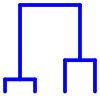
\includegraphics[width=1cm]{testtree1} & $\times$ 10 &
      $\cdots$ &
      
\includegraphics[width=1cm]{testtree3} & $\times$ 10
    \end{tabular}
  };

  \node (rect4) [box, below=of rect2] { };
  \node at (rect4.north) [anchor=north] {\uline{$15 \times n$ training trees}};
  \node [above=4pt of rect4.south] {
    \begin{tabular}{m{0.8cm} m{1cm} m{1cm} m{0.8cm} m{1cm}}
      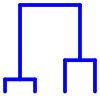
\includegraphics[width=1cm]{testtree1} & $\times$ 15 &
      $\cdots$ &
      
\includegraphics[width=1cm]{testtree3} & $\times$ 15
    \end{tabular}
  };

  \coordinate [left=0.5 of rect4.south west] (r4sw);
  \node (rect5) [box, below=of r4sw] { };
  \node at (rect5.north) [anchor=north] {\uline{$10 \times k$ kernel score vectors}};
  \node [above=0 of rect5.south, minimum width=\boxw, align=center] {
    \includegraphics[scale=0.6]{tinykscore}
  };

  \node (rect6) [box, below=of rect5] { };
  \node at (rect6.north) [anchor=north] {\uline{$10 \times k$ parameter estimates}};
  \node [above=6pt of rect6.south, minimum width=\boxw, text width=\boxw, align=center] {
    point estimate = training value with highest median kernel score
  };

  \coordinate [above=0.5 of rect5.north] (r5n);
  \draw [next] (rect1) -- (rect3);
  \draw [next] (rect2) -- (rect4);
  \draw [next] (rect3) |- (r5n) -- (rect5);
  \draw [next] (rect4) |- (r5n) -- (rect5);
  \draw [next] (rect5) -- (rect6);

\end{tikzpicture}

\end{document}
